\documentclass[12pt,twoside]{article}
%\documentclass[10pt,twoside,twocolumn]{article}
\usepackage[english]{babel}
\usepackage{times,subeqnarray}
\usepackage{url}
% following is for pdflatex vs. old(dvi) latex
\newif\myifpdf
\ifx\pdfoutput\undefined
%  \pdffalse           % we are not running PDFLaTeX
   \usepackage[dvips]{graphicx}
\else
   \pdfoutput=1        % we are running PDFLaTeX
%  \pdftrue
   \usepackage[pdftex]{graphicx}
\fi
\usepackage{apatitlepages}
% if you want to be more fully apa-style for submission, then use this
%\usepackage{setspace,psypub,ulem}
%\usepackage{setspace} % must come before psypub
%\usepackage{psypub}
%\usepackage{psydraft}
\usepackage{one-in-margins}  % use instead of psydraft for one-in-margs
\usepackage{scicite}
%\usepackage{apa}       % apa must come last
% using latex2e as standard, use the following for latex209
% \documentstyle [times,11pt,twoside,subeqnarray,psydraft,apa,epsf]{article}
%\input netsym

% tell pdflatex to prefer .pdf files over .png files!!
\myifpdf
  \DeclareGraphicsExtensions{.pdf,.eps,.png,.jpg,.mps,.tif}
\fi

\newenvironment{sciabstract}{%
\begin{quote}}
{\end{quote}}

\renewcommand\refname{References and Notes}

\newcounter{lastnote}
\newenvironment{scilastnote}{%
\setcounter{lastnote}{\value{enumiv}}%
\addtocounter{lastnote}{+1}%
\begin{list}%
{\arabic{lastnote}.}
{\setlength{\leftmargin}{.22in}}
{\setlength{\labelsep}{.5em}}}
{\end{list}}

% use 0 for psypub format 
\parskip 2pt
% for double-spacing, determines spacing 
%\doublespacing
%\setstretch{1.7}

\columnsep .25in   % 3/8 in column separation

\def\myheading{ Deep Predictive Learning }

% no twoside for pure apa style, use \markright with heading only
\pagestyle{myheadings}
\markboth{\hspace{.5in} \myheading \hfill}{\hfill O'Reilly, Russin, \& Rohrlich \hspace{.5in}}

\bibliographystyle{Science}

\title{ {\bf Title:} Deep Predictive Learning as a Model of Human Learning } 

\author{{\bf Authors:} Randall C. O'Reilly,$^\ast$ Jacob L. Russin, and John Rohrlich\\
\vspace{.15in}\\
  {\bf Affiliations:} Departments of Psychology and Computer Science\\
  Center for Neuroscience\\
  University of California, Davis \\
  \vspace{.15in}\\
  $^\ast$Correspondence to: \texttt{oreilly@ucdavis.edu}\\
  1544 Newton Ct\\
  Davis, CA 95616\\
  \\}

\begin{document}

% sloppy is the way to go!
\sloppy
\raggedbottom
%\baselineskip20pt

\maketitle 

\begin{sciabstract}
{\bf Abstract:} Understanding the principles underlying the power of human learning is a widely held goal of research in machine learning, yet these models unrealistically rely on massive human-labeled datasets.  We present a biologically based model of predictive learning, which generates predictions at the alpha frequency (10 Hz), and learns from prediction errors, requiring no labeled inputs.  Distinctive patterns of connectivity between the neocortex and thalamus drive alternating top-down prediction and bottom-up outcome representations over the pulvinar nucleus, with the temporal difference driving error-driven learning throughout neocortex.  However, can it learn abstractions that go beyond the surface input level?  Our model does, in ways that match both human category representations and monkey electrophysiology, while comparison models lacking biological features do not.

{\bf One Sentence Summary:} The human brain learns from prediction errors generated on the pulvinar nucleus, and a model thereof develops abstract knowledge.

\end{sciabstract}

\clearpage

\pagestyle{myheadings}

The success of deep convolutional neural networks (DCNN's) \cite{KrizhevskySutskeverHinton12,LeCunBengioHinton15,Schmidhuber15a} in object recognition and many other domains raises the question of how well they model human learning, at both neural and cognitive levels.  Although the engine of these models, error backpropagation \cite{RumelhartHintonWilliams86}, has long been questioned on biological grounds \cite{Crick89}, various related biologically plausible mechanisms have been proposed \cite{OReilly96,XieSeung03,BengioMesnardFischerEtAl17}.  However, the need for massive amounts of labeled data still makes these models cognitively implausible: non-human primates and infants learn to recognize and categorize objects without the benefit of such labeled data \cite{LakeUllmanTenenbaumEtAl17}.  An alternative, biologically plausible approach is to use {\em predictive error-driven learning}, where error signals arise from differences between a prediction of what will happen next, and what actually does occur \cite{Elman90,ElmanBatesKarmiloff-SmithEtAl96}.  In principle, all that this requires is: 1) events to unfold over time; 2) a learning system that is somehow organized to generate predictions of these events; and 3) a biological mechanism that learns from prediction errors. Furthermore, a system that learned to accurately predict complex real-world events would require considerable knowledge to have been acquired in the process of so doing, and thus there is reason to believe that predictive learning could power sophisticated, important forms of developmental learning.

Here we show that canonical circuits between the neocortex and thalamus have several distinctive properties that directly support predictive error-driven learning.  When implemented in a computational model employing a biologically plausible form of error backpropagation \cite{OReilly96,OReillyMunakata00,OReillyMunakataFrankEtAl12}, along with several other important properties of the mammalian visual system, the model learns to systematically categorize 3D objects according to invariant shape properties.  Furthermore, this category structure matches human judgments of these same objects, and is consistent with neural representations in inferotemporal (IT) cortex in primates.  Comparison models with the same architecture but using standard non-biological error-backpropagation learning, and models using the state-of-the-art {\em PredNet} predictive learning architecture \cite{LotterKreimanCox16}, support the idea that predictive learning is useful for shaping internal representations, but these models do not learn much beyond the similarities present at the lowest visual levels.  Thus, we argue that incorporating biological properties of the brain can potentially provide a better understanding of human learning at multiple levels relative to existing DCCN models.

\begin{figure}
  \centering\includegraphics[width=6in]{figs/fig_deepleabra_wwi_abc_pred_model_frames}
  \caption{\footnotesize {\bf a)} Schematic illustration of the temporal evolution of information flow in the DeepLeabra framework predicting visual sequences, over two alpha cycles of 100 msec each.  During each alpha cycle, the V2 Deep layer (cortical lamina 5, 6) uses the prior 100 msec of context information to generate a prediction (minus phase) over the pulvinar thalamic relay cell (TRC) neurons, of what will happen next.  The bottom-up actual outcome is driven over the pulvinar via the 5IB strong driver inputs from V1, providing the {\em plus} or {\em target} phase of learning.  Error-driven learning occurs as a function of the {\em temporal difference} between the plus and minus activation states, in both superficial (lamina 2, 3) and deep layers, via the pulvinar projections into these layers.  The 5IB bursting in V2 drives an update of the local temporal context information in V2 Deep layers, which is used in generating the minus phase prediction in the next alpha cycle, and so on.  These same 5IB cells drive a plus phase in higher area TRC's as well, which perform the same kind of {\em local} predictive auto-encoder learning as shown for V2 here.  See supplementary material for more details. {\bf b)} The three-visual-stream deep predictive learning model ({\em What-Where-Integration, WWI} model). The dorsal {\em Where} pathway learns first, using easily-abstracted {\em spatial blobs}, to predict where an object will move next, based on prior motion history, visual motion, and saccade efferent copy signals.  This drives strong top-down inputs to lower areas with accurate spatial predictions, leaving the {\em residual} error concentrated on {\em What} and {\em What * Where} integration information.  The V3 and DP (dorsal prelunate) areas constitute the {\em What * Where} integration pathway, helping bind features and locations.  V4, TEO, and TE are the {\em What} pathway, learning abstracted object category representations, which also drive strong top-down inputs to lower areas.  {\em s} suffix = superficial layer, {\em d} = deep layer, and {\em p} = pulvinar. {\bf c)} An example sequence of 8 frames (8 alpha cycles) that the model learned to predict (the car is moving steadily up, and rotating in depth, with saccades recentering it on the ``retina''), with the reconstruction of each image based on the V1 gabor filters ({\em V1h recon}), and a reconstruction of the model-generated prediction for each frame over the higher resolution V1hp pulvinar layer (to compare against V1h recon, correlation value $r$ shown).  The relatively low resolution encoding of the image makes these somewhat difficult to interpret, but the $r$ values are well above the $r$'s for each V1 state compared to the previous time step (mean = .38, min of .16 on frame 4 when the prediction is at .57 -- see supplementary material for more analysis), indicating that the model has learned somewhat vague but broadly accurate predictions that go well beyond e.g., just copying the previous time step.  The eye icons indicate when a saccade occurred.}
  \label{fig.model}
\end{figure}

Motivated by biological evidence, we hypothesize that sensory predictions in posterior neocortex are generated roughly every 100 msec (i.e., the {\em alpha} rhythm, 10 Hz), by neurons in the deep layers of the neocortex that project to the pulvinar nucleus of the thalamus (Figure~\ref{fig.model}a) \cite{OReillyWyatteRohrlich14}.  The pulvinar represents this top-down prediction for roughly 75 msec of the alpha cycle as it develops, after which point the layer 5IB intrinsic-bursting neurons send strong, bottom-up driving input to the pulvinar, representing the actual sensory stimulus \cite{ShermanGuillery06}.  These 5IB neurons burst at the alpha frequency, determining the overall timing of the predictive learning cycle, along with other dynamic parameters of the thalamocortical circuit \cite{LorinczKekesiJuhaszEtAl09,FranceschettiGuatteoPanzicaEtAl95,SaalmannPinskWangEtAl12}.  The prediction error is implicit in the temporal difference between these two periods of activity within the alpha cycle over the pulvinar, which is consistent with the biologically plausible form of error-driven cortical learning used in our models \cite{OReilly96}.  The pulvinar sends broad projections back up to all of the areas that drive top-down predictions into it \cite{Shipp03,Mumford91}, thus broadcasting this error signal to drive local synaptic plasticity in the neocortex. Mathematically, this approximates gradient descent to minimize overall prediction errors.  This computational framework makes sense of otherwise puzzling anatomical and physiological properties of the cortical and thalamic networks \cite{ShermanGuillery06}, and is consistent with a wide range of detailed neural and behavioral data regarding the effects of the alpha rhythm on learning and perception \cite{BuffaloFriesLandmanEtAl11,VanRullenKoch03,JensenBonnefondVanRullen12,FiebelkornKastner19}.  It has many testable differences from other existing theories of predictive learning that have been proposed over the years, at varying levels of biological detail \cite{Mumford92,RaoBallard99,KawatoHayakawaInui93,Friston05}.

A critical question for predictive learning is whether it can develop high-level, abstract ways of representing the raw sensory inputs, while learning from nothing but predicting these low-level visual inputs.  For example, can predictive learning really eliminate the need for human-labeled image datasets where abstract category information is explicitly used to train object recognition models via error-backpropagation?  From a cognitive perspective, there is considerable evidence that non-verbal primates, and pre-verbal human infants, naturally develop abstract categorical encodings of visual objects in IT cortex \cite{CadieuHongYaminsEtAl14}, without relying on any explicit external categorical labels.  Existing predictive-learning models based on error backpropagation \cite{LotterKreimanCox16} have not demonstrated the development of abstract, categorical representations.  Also, the more prevalent test is on their ability to subsequently train using the human-generated labels, but there are many ways in which prior training could facilitate such training without fully forming systematic categories {\em de-novo}.

To determine if our biologically based predictive learning model (Figure~\ref{fig.model}b) can naturally form such categorical encodings in the complete absence of external category labels, we showed the model brief movies of 156 3D object exemplars drawn from 20 different basic-level categories (e.g., car, stapler, table lamp, traffic cone, etc.) selected from the CU3D-100 dataset \cite{OReillyWyatteHerdEtAl13}.  The objects moved and rotated in 3D space over 8 movie frames, where each frame was sampled at the alpha frequency (Figure~\ref{fig.model}c).  There were also saccadic eye movements every other frame, with an efferent copy signal to enable full prediction of the effects of the eye movement, which allows the model to capture predictive remapping (a widely-studied signature of predictive learning in the brain) \cite{DuhamelColbyGoldberg92,CavanaghHuntAfrazEtAl10}, and introduces additional predictive-learning challenge.  The only learning signal available to the model was the temporal difference prediction error between what it predicted to see in the next frame, compared to what was actually seen.  

\begin{figure}
  \centering\includegraphics[width=6in]{figs/fig_deepleabra_wwi_rsa_leabra_expt1}
  \caption{\small {\bf a)} Category similarity structure that developed in the highest layer, TE, of the biologically based predictive learning model, showing {\em 1-correlation} similarity of the TE representation for each 3D object against every other 3D object (156 total objects). Blue cells have high similarity, and model has learned block-diagonal clusters or categories of high-similarity groupings, contrasted against dissimilar (yellow) off-diagonal other categories.  Clustering maximized the overall average {\em within - between} correlation distance across given set of clusters (see supplementary materials for details).  Note that all items from the same ``objective'' basic-level object categories (N=20) are reliably sorted within a given learned category, so these categories subsume our more fine-grained object categories. {\bf b)} Human similarity ratings for the same 3D objects, presented with the V1 reconstruction (see Fig 1c) to capture coarse perception in our model, aggregated at the level of the 20 basic-level categories since we could not sample the entire 156 x 156 matrix. Each cell is 1 - proportion that the given pair of objects was rated as more similar than another pair of objects (see supplementary material for details of the experiment).  The resulting similarity matrix generally exhibits the same categorical structure as the model (confirmed by permutation testing and agglomorative cluster analysis).  {\bf c)} Emergence of abstract category structure over the hierarchy of layers.  Red line shows correlation similarity between the similarity matrix for TE (shown in panel a) against the similarity matrix computed for every other layer, and the black line shows the correlation similarity for the V1 layer matrix against every other layer (1 = identical; 0 = orthogonal). Both show that IT layers (TEO, TE) progressively differentiate from raw input similarity structure present in V1, and, critically, that the model has learned structure beyond that present in the input.}
  \label{fig.rsa}
\end{figure}

We performed a representational similarity analysis (RSA) on the learned activity patterns at each layer in the model, and found that the highest IT layer (TE) produced a systematic organization of the 156 3D objects into 5 categories (Figure~\ref{fig.rsa}a), which visually correspond to the overall shape of the objects (pyramid-shaped, vertically-elongated, round, boxy / square, and horizontally-elongated). This organization of the objects matches that produced by humans making shape similarity judgments on the same set of objects, using the V1 reconstruction as shown in Figure~\ref{fig.model}c to capture the model's coarse-grained perception (Figure~\ref{fig.rsa}b; see supplementary material for methods and further analysis).  Critically, Figure~\ref{fig.rsa}c shows that the overall similarity structure present in IT layers (TEO, TE) of the biological model is significantly different from the similarity structure at the level of the V1 primary visual input.  Thus the model, despite being trained only to generate accurate visual input-level predictions, has learned to represent these objects in an abstract way that goes beyond the raw input-level information.  Furthermore, because this abstract category organization reflects the overall visual shapes of the objects as judged by human participants, this suggests that the model is extracting the overall geometrical shape information that is apparent once these objects are encoded in an invariant way independent of motion, rotation, and scaling transformations present in the V1 visual inputs.  We further verified that at the highest IT levels in the model, a consistent, spatially-invariant representation is present across different views of the same object (e.g., the average correlation across frames within an object was .901).  This is also evident in Figure~\ref{fig.rsa}a by virtue of the close similarity across multiple objects within the same category.

\begin{figure}
  \centering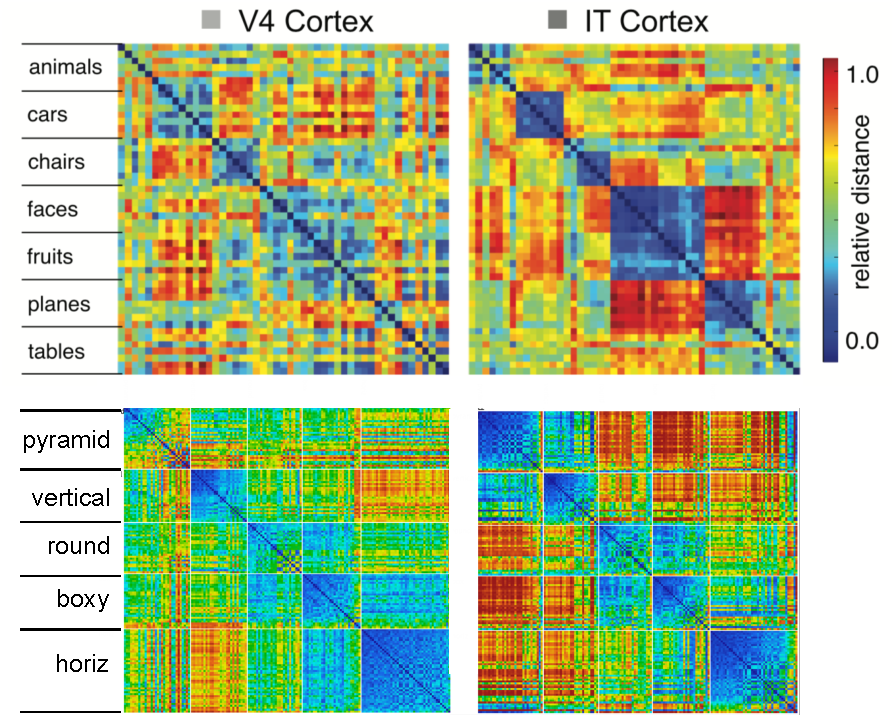
\includegraphics[width=4in]{figs/fig_deepleabra_wwi_rsa_leabra_macaque}
  \caption{\small Comparison of progression from V4 to IT in macaque monkey visual cortex (top row, from Cadieu et al, 2014) versus same progression in model (replotted using comparable color scale).  Although the underlying categories are different, and the monkeys have a much richer multi-modal experience of the world that could help reinforce categories such as foods and faces, our model nevertheless shows a similar qualitative progression in extent of stronger categorical structure in IT, where the block-diagonal highly similar representations are more consistent across categories, and the off-diagonal differences are stronger and more consistent as well (i.e., categories are also more clearly differentiated).  Note that the critical difference in our model versus those compared in Cadieu et al 2014 and related papers is that they explicitly trained their models on category labels, whereas our model is {\em entirely self-organizing} and has no external categorical training signal.}
  \label{fig.macaque}
\end{figure}

Further evidence for the progressive nature of representation development in our model is shown in Figure~\ref{fig.macaque}, which compares the similarity structures in layers V4 and IT in macaque monkeys \cite{CadieuHongYaminsEtAl14} with those in corresponding layers in our model.  In both the monkeys and our model, the higher IT layer builds upon and clarifies the noisier structure that is emerging in the earlier V4 layer.  Considerable other work has also compared DCNN representations with these same data from monkeys \cite{CadieuHongYaminsEtAl14}, but it is essential to appreciate that those DCNN models were explicitly trained on the category labels, making it somewhat less than surprising that such categorical representations developed.  By contrast, we reiterate that our model has discovered its categorical representations entirely on its own, with no explicit categorical inputs or training of any kind.

\begin{figure}
  \centering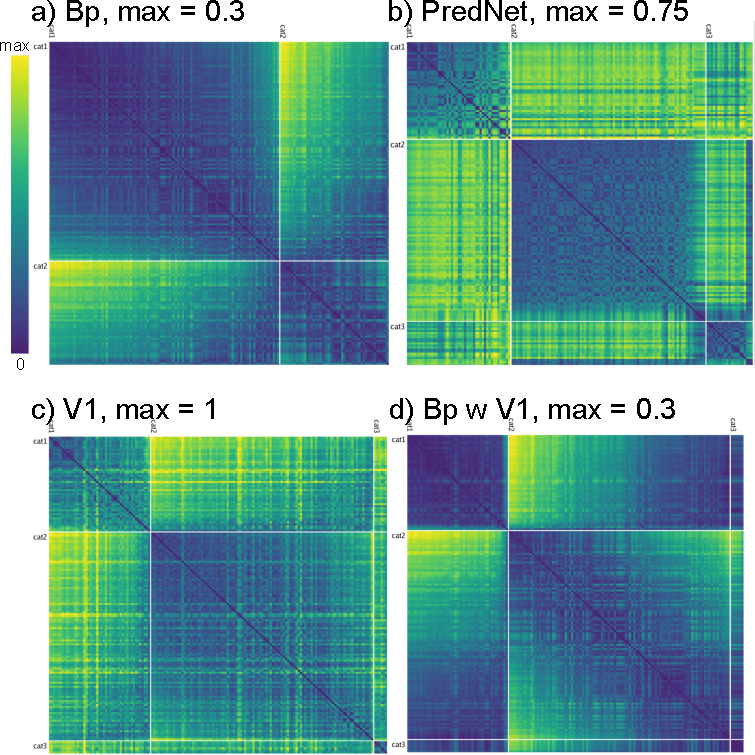
\includegraphics[width=4.5in]{figs/fig_deepleabra_wwi_bp_prednet_simat}
  \caption{\small {\bf a)} Category similarity structure in the highest IT layer (TE) of the backpropagation (Bp) model with the same What / Where structure.  Only two broad categories are present, and the lower {\em max} distance (0.3 vs. 1.5 in biological model) indicates that overall the patterns are highly similar.  {\bf b)} Similarity structure for the PredNet model, in the highest of its layers (layer 3), which is even less differentiated (max = 0.15) but overall follows the same broad category structure.  {\bf c)} Comparison of similarity structures across layers in the Bp model (compare to Figure~2c): unlike in the biological model, the V1 structure is largely preserved across layers, and is little different from the structure that best fits the TE layer shown in panel a, indicating that the model has not developed abstractions beyond the structure present in the visual input.  Layer V3 is most directly influenced by spatial prediction errors in its connections with the dorsal pathway, so it differs from both in strongly encoding position information.  {\bf d)} The best fitting V1 structure, which has 2 broad categories and banana is in a third category by itself.  The lack of dark blue on the block diagonal indicates that these categories are overall quite weak, and every item is fairly dissimilar from every other.  {\bf e)} The same similarities shown in panel a for Bp TE also fit reasonably well in the V1 structure (and they have a similar average within - between contrast differences, of 0.0838 and 0.0513).  {\bf f)} The similarity structure from the biological model does {\em not} fit well within the V1 organization (the blue is not consistently aligned along the block diagonal, and the yellow is not strictly off-diagonal), consistent with the large difference in average contrast distance (0.5071 for the best categories vs. 0.3070 for the V1 categories).}
  \label{fig.bpred}
\end{figure}

Figure~\ref{fig.bpred} shows the results from a purely backpropagation-based version of the same model architecture.  In this model, the highest layers in the network form a simple binary category structure overall, and the detailed item-level similarity structure does not diverge significantly from that present at the lowest V1 inputs, indicating that it has not formed novel systematic structured representations, in contrast to those formed in the biologically based model.  Thus, it is clear that the additional biologically motivated properties of the original model are playing a critical role in the development of abstract categorical representations. These properties include: excitatory bidirectional connections, inhibitory competition, and an additional Hebbian form of learning that serves as a regularizer (similar to weight decay) on top of predictive error-driven learning \cite{OReilly98,OReillyMunakata00}.

Each of these properties could promote the formation of categorical representations. Bidirectional connections enable top-down signals to consistently shape lower-level representations, creating significant attractor dynamics that cause the entire network to settle into discrete categorical attractor states. By contrast, backpropagation networks typically lack these kinds of attractor dynamics, and this could contribute significantly to their relative lack of categorical learning.  Hebbian learning drives the formation of representations that encode the principal components of activity correlations over time, which can help more categorical representations coalesce (and results below already indicate its importance).  Inhibition, especially in combination with Hebbian learning, drives representations to specialize on more specific subsets of the space.  Ongoing work is attempting to determine which of these is essential in this case (perhaps all of them) by systematically introducing some of these properties into the backpropagation model, though this is difficult because full bidirectional recurrent activity propagation, which is essential for conveying error signals top-down in the biological network, is incompatible with the standard efficient form of error backpropagation, and requires much more computationally intensive and unstable forms of fully recurrent backpropagation \cite{WilliamsZipser92,Pineda87}.  Furthermore, Hebbian learning requires inhibitory competition which is difficult to incorporate within the backpropagation framework.

\begin{figure}
  \centering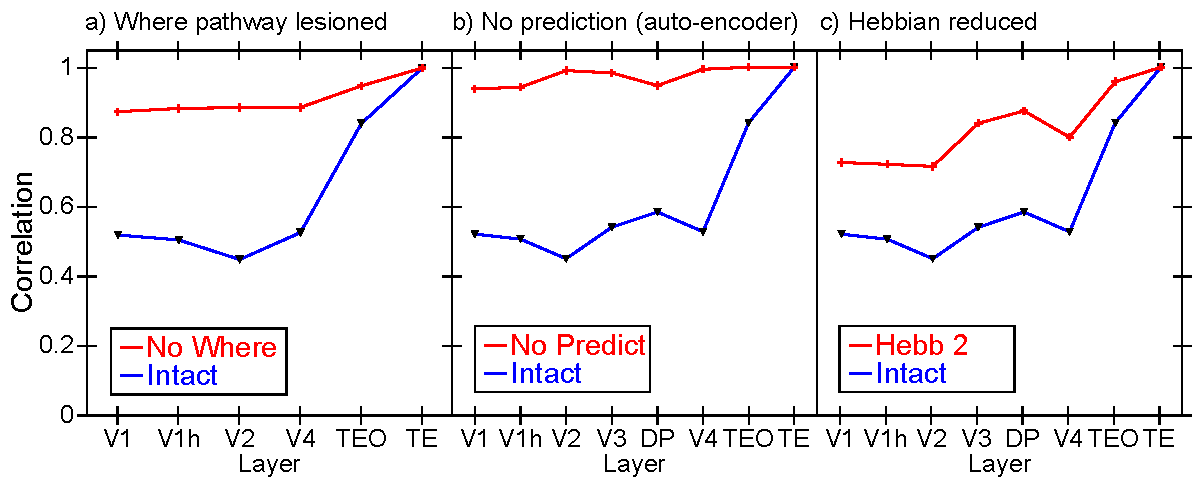
\includegraphics[width=4in]{figs/fig_deepleabra_wwi_leabra_manips}
  \caption{\small Effects of various manipulations on the extent to which the TE layer representations differentiate from the V1 structure.  {\em Std} is the same result shown in Figure 2c from the intact model (see caption there for further explanation), and all manipulations significantly impair the development of abstract TE categorical representations (i.e., the TE representations are more similar to V1 and the other layers).  {\bf a)} Dorsal {\em Where} pathway lesions, including lateral inferior parietal sulcus (LIP), V3, and dorsal prelunate (DP).  This pathway is essential for regressing out location-based prediction errors, so that the residual errors concentrate feature-encoding errors that train the {\em What} pathway.  {\bf b)} Allowing the deep layers full access to current-time information, thus effectively eliminating the prediction demand and turning the network into an auto-encoder, which significantly impairs representation development, and supports the importance of the challenge of predictive learning for developing deeper, more abstract representations.  {\bf c)} Reducing the strength of Hebbian learning from 2.5 to 2, demonstrating the essential role played by this form of learning on shaping categorical representations.  Eliminating Hebbian learning entirely prevented the model from learning anything at all, as it also plays a critical regularization and shaping role on learning.}
  \label{fig.manips}
\end{figure}

Figure~\ref{fig.manips} shows just a few of the large number of parameter manipulations that have been conducted to develop and test the final architecture.  For example, we hypothesized that separating the overall prediction problem between a spatial {\em Where} vs. non-spatial {\em What} pathway \cite{UngerleiderMishkin82,GoodaleMilner92}, would strongly benefit the formation of more abstract, categorical object representations in the {\em What} pathway.  Specifically, the {\em Where} pathway can learn relatively quickly to predict the overall spatial trajectory of the object (and anticipate the effects of saccades), and thus effectively regress out that component of the overall prediction error, leaving the residual error concentrated in object feature information, which can train the ventral {\em What} pathway to develop abstract visual categories.  Figure~\ref{fig.manips}a shows that, indeed, when the {\em Where} pathway is lesioned, the formation of abstract categorical representations in the intact {\em What} pathway is significantly impaired.  Figure~\ref{fig.manips}b shows that full predictive learning, as compared to just encoding and decoding the current state (which is much easier computationally, and leads to much better overall accuracy), is also critical for the formation of abstract categorical representations --- prediction is a ``desirable difficulty'' \cite{Bjork94}.  Finally, Figure~\ref{fig.manips}c shows the impact of reducing Hebbian learning, which impairs category learning as expected.

In conclusion, we have demonstrated that learning based strictly on predicting what will be seen next is, in conjunction with a number of critical biologically motivated network properties and mechanisms, capable of generating abstract, invariant categorical representations of the overall shapes of objects.  The nature of these shape representations closely matches human shape similarity judgments on the same objects.  Thus, predictive learning has the potential to go beyond the surface structure of its inputs, and develop systematic, abstract encodings of the ``deeper'' structure of the environment.  Relative to existing machine-learning-based approaches in ``deep learning'', which have generally focused on raw categorization accuracy measures using explicit category labels or other human-labeled inputs, the results here suggest that focusing more on the nature of what is learned in the model might provide a valuable alternative approach.  Considerable evidence in cognitive neuroscience suggests that the primary function of the many nested (``deep'') layers of neural processing in the neocortex is to {\em simplify} and aggressively {\em discard} information \cite{SimonsRensink05}, to produce precisely the kinds of extremely valuable abstractions such as object categories, and, ultimately, symbol-like representations that support high-level cogntive processeses such as reasoning and problem-solving \cite{RougierNoelleBraverEtAl05,OReillyPetrovCohenEtAl14}.  Thus, particularly in the domain of predictive or generative learning, the metric of interest should not be the accuracy of prediction itself (which is indeed notably worse in our biologically based model compared to the DCNN-based PredNet and backpropagation models), but rather whether this learning process results in the formation of simpler, abstract representations of the world that can in turn support higher levels of cognitive function.

Considerable further work remains to be done to more precisely characterize the essential properties of our biologically motivated model necessary to produce this abstract form of learning, and to further explore the full scope of predictive learning across different domains.  We strongly suspect that extensive cross-modal predictive learning in real-world environments, including between sensory and motor systems, is a significant factor in infant development and could greatly multiply the opportunities for the formation of higher-order abstract representations that more compactly and systematically capture the structure of the world \cite{YuSmith12}.  Future versions of these models could thus potentially provide novel insights into the fundamental question of how deep an understanding a pre-verbal human, or a non-verbal primate, can develop \cite{SpelkeBreinlingerMacomberEtAl92,ElmanBatesKarmiloff-SmithEtAl96}, based on predictive learning mechanisms.  This would then represent the foundation upon which language and cultural learning builds, to shape the full extent of human intelligence.

\bibliography{ccnlab}

\section*{Acknowledgements}

We thank Dean Wyatte, Tom Hazy, Seth Herd, Kai Krueger, Tim Curran, David Sheinberg, Lew Harvey, Jessica Mollick, Will Chapman, Helene Devillez, and the rest of the CCN Lab for many helpful comments and suggestions.

  {\bf Funding:} Supported by: ONR grants ONR N00014-19-1-2684 / N00014-18-1-2116, N00014-14-1-0670 / N00014-16-1-2128, N00014-18-C-2067, N00014-13-1-0067, D00014-12-C-0638.  This work utilized the Janus supercomputer, which is supported by the National Science Foundation (award number CNS-0821794) and the University of Colorado Boulder. The Janus supercomputer is a joint effort of the University of Colorado Boulder, the University of Colorado Denver and the National Center for Atmospheric Research.

 {\bf Author Contributions:} RCO developed the model, performed the non-PredNet simulations, and drafted the paper. JLW performed the PredNet simulations and analysis, and edited the paper.  JR contributed to developing the model and edited the paper.

  {\bf Competing Interests:} R. C. O'Reilly is Chief Scientist at eCortex, Inc., which may derive indirect benefit from the work presented here.

{\bf Data and Materials Availability:}  All data and materials will be available at \url{https://github.com/ccnlab/deep-obj-cat} upon publication.

\section*{Supplementary materials}

Materials and Methods

Figures S1 - ?

\end{document}
